\documentclass[convert={size=150,outext=.png}]{standalone}
\usepackage{graphicx}
\usepackage{epstopdf}
%\usepackage{hyperref}
%\usepackage{color}

%\usepackage[T1]{fontenc}
%\usepackage{mathpazo}

%\setlength{\parindent}{0cm}

\usepackage{tikz}
%\usetikzlibrary{calc,intersections,patterns}

\begin{document}
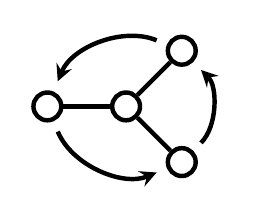
\begin{tikzpicture}
	[inner sep=1.25mm,
	 knot/.style={circle,draw,ultra thick},
	 arrow/.style={->,>=stealth,shorten >=4,shorten <=4,ultra thick},
	 line/.style={-,ultra thick}]

	\path [use as bounding box] (-1.25,-1.1) rectangle (1.25,1);
	
	\node[knot] (centre)   at (0,0) {};
	\node[knot] (left)     at (180:1) {};
	\node[knot] (topright) at (45:1) {};
	\node[knot] (botright) at (-45:1) {};
	
	\draw[line] (centre) -- (left);
	\draw[line] (centre) -- (topright);
	\draw[line] (centre) -- (botright);
	
	\draw[arrow] (left)     to [bend right=45] (botright);
	\draw[arrow] (botright) to [bend right=45] (topright);
	\draw[arrow] (topright) to [bend right=45] (left);
\end{tikzpicture}

\end{document}